\documentclass{article}
\usepackage[final]{nips_2017}
\usepackage{polski}
\usepackage[utf8]{inputenc}    % allow utf-8 input
\usepackage[T1]{fontenc}       % use 8-bit T1 fonts
\usepackage{hyperref}          % hyperlinks
\usepackage{url}               % simple URL typesetting
\usepackage{booktabs}          % professional-quality tables
\usepackage{amsfonts}          % blackboard math symbols
\usepackage{nicefrac}          % compact symbols for 1/2, etc.
\usepackage{microtype}         % microtypography
\usepackage[section]{placeins} % figures kept in sections
\usepackage{graphicx}          % images
\graphicspath{ {./img/} }
\usepackage{multirow}
\usepackage{float}             % figures in place
\usepackage{caption}		   % smaller margin after figure

\renewcommand{\figurename}{Wykres}
\setlength{\belowcaptionskip}{-20pt}

\title{  Sieć wielowarstwowa\\Sieci Neuronowe 2020 }

\author{
  Jakub Ciszek \\
  238035\\
}

\begin{document}

\maketitle

\newpage
\tableofcontents
\newpage

Cały kod wykorzystany w zadaniu znajduje się pod adresem: \url{https://github.com/Greenpp/sieci-neuronowe-pwr-2020}

\section{Opis badań}
\subsection{Plan eksperymentów}

Wszystkie eksperymenty zostały przeprowadzone 10 razy. Losowość przy inicjalizacji wag oraz generacji danych nie została narzucona żadnym ziarnem. Podczas badań przyjęto górną granicę 5 epok, po przekroczeniu której, uczenie zostawało przerywane. Ze względu na charakter zadania (klasyfikacja) na ostatniej warstwie użyto funkcji Softmax, a za funkcję straty przyjęto Entropię krzyżową.
Z powodów wydajnościowych testowanie modelu przeprowadzano co każde 1024 przykłady, niezależnie od wielkości paczki.\\
Zgodnie z instrukcją zostały przeprowadzone następujące badania:
\begin{itemize}
	\item Wpływ wielkości warstwy ukrytej na przebieg procesu uczenia
	\item Wpływ wielkości paczki na przebieg procesu uczenia
	\item Wpływ zakresu inicjalizacji wag na przebieg procesu uczenia
	\item Wpływ wartości współczynnika alpha na przebieg procesu uczenia
	\item Wpływ użytej funkcji aktywacyjnej na przebieg procesu uczenia     
\end{itemize}
Podczas wizualizacji funkcji straty pominięto pierwsze 10 pomiarów dla lepszej czytelności.

\subsection{Charakterystyka zbiorów danych}

Danymi użytymi w zadaniu jest zbiór ręcznie pisanych cyfr \(0-9\) - MNIST. Na zbiór składa się 70,000 obrazów wielkości 28x28 pikseli, co po przekształceniu odpowiadało 784 elementowemu wektorowi wejściowemu i 10 klasom na wyjściu. Użyta w zadaniu wersja została podzielona na 3 zbiory:
\begin{itemize}
	\item Uczący - 50,000 przykładów.
	\item Walidujący - 10,000 przykładów.
	\item Testowy - 10,000 przykładów.
\end{itemize}
W trakcie eksperymentów wykorzystano jedynie zbiory uczący i testowy.

\newpage
\section{Eksperymenty}

\subsection{Wpływ wielkości warstwy ukrytej na przebieg procesu uczenia}
\subsubsection*{Założenia}
\begin{table}[H]
	\caption{Stałe dla eksperymentu 1}
	\label{tabela-const-1}
	\centering
	\begin{tabular}{lr}
		\toprule
		Parametr               & Wartość         \\
		\midrule
		Wielkość paczki      & 32                \\
		Zakres wag             & \($-0.5 -- 0.5$\) \\
		Współczynnik uczenia & 0.01              \\
		Funkcja aktywacji      & ReLU              \\
		\bottomrule
	\end{tabular}
\end{table}

Zmienną w tym eksperymencie była wielkość warstwy ukrytej. Ilość neuronów przyjmowała wartości ze zbioru \(\{$16, 128, 512, 2048$\}\)
\subsubsection*{Przebieg}

Podczas eksperymentu model został zainicjalizowany 10 razy dla każdej z badanych wartości oraz wyuczony, uzyskane wyniki zostały zapisane w postaci pliku .plk do dalszej analizy.

\subsubsection*{Wyniki}
\begin{figure}[H]
	\centering
	\caption{Dokładność modelu w zależności od wielkości warstwy ukrytej}
	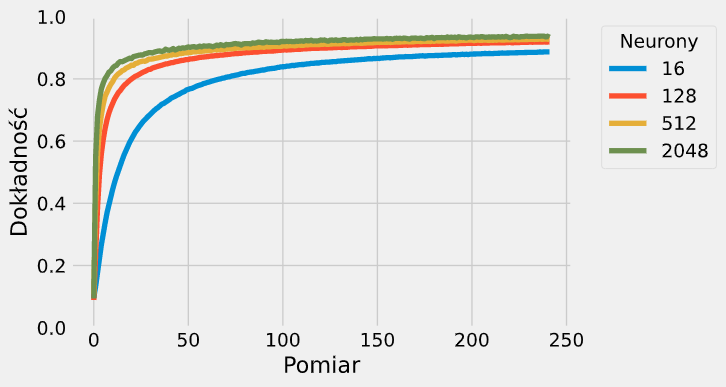
\includegraphics[width=\textwidth]{hidden_acc.png}
	\label{fig:res11}
\end{figure}
\begin{figure}[H]
	\centering
	\caption{Dokładność modelu w końcowym etapie uczenia w zależności od wielkości warstwy ukrytej}
	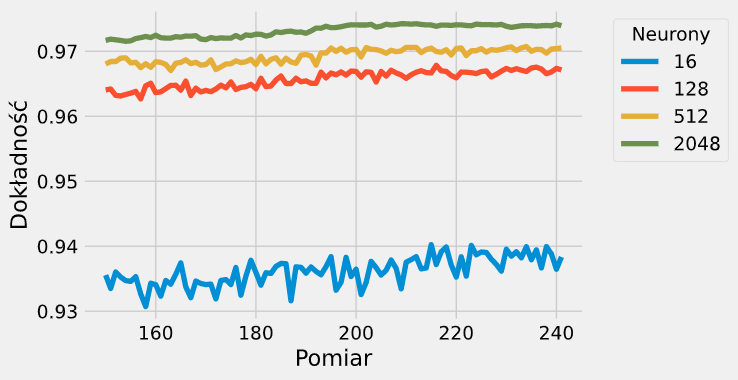
\includegraphics[width=\textwidth]{hidden_acc_zoom.png}
	\label{fig:res12}
\end{figure}
\begin{figure}[H]
	\centering
	\caption{Zachowanie funkcji błędu dla 16 neuronów}
	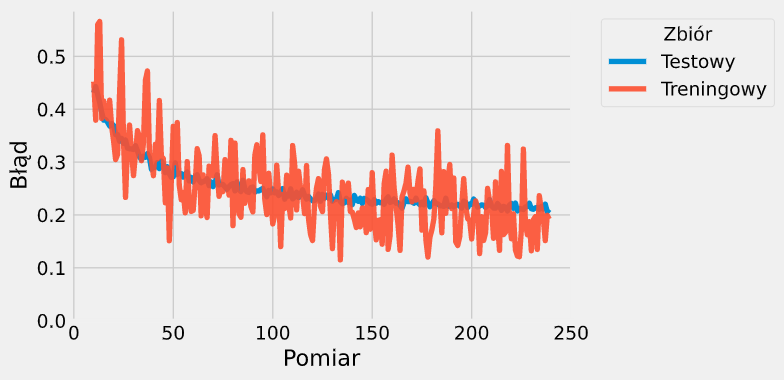
\includegraphics[width=\textwidth]{hidden_err_16.png}
	\label{fig:res13}
\end{figure}
\begin{figure}[H]
	\centering
	\caption{Zachowanie funkcji błędu dla 128 neuronów}
	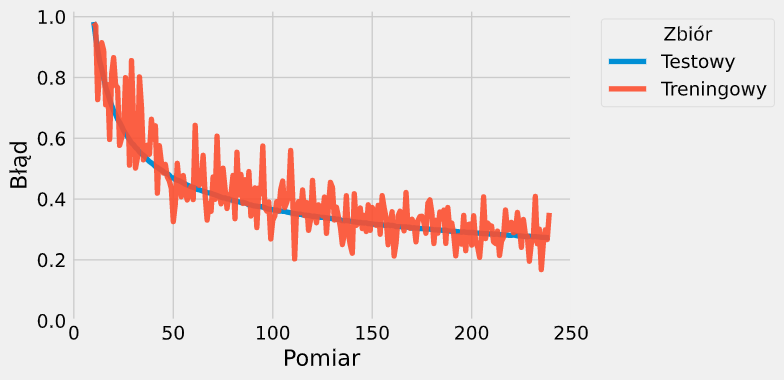
\includegraphics[width=\textwidth]{hidden_err_128.png}
	\label{fig:res14}
\end{figure}
\begin{figure}[H]
	\centering
	\caption{Zachowanie funkcji błędu dla 512 neuronów}
	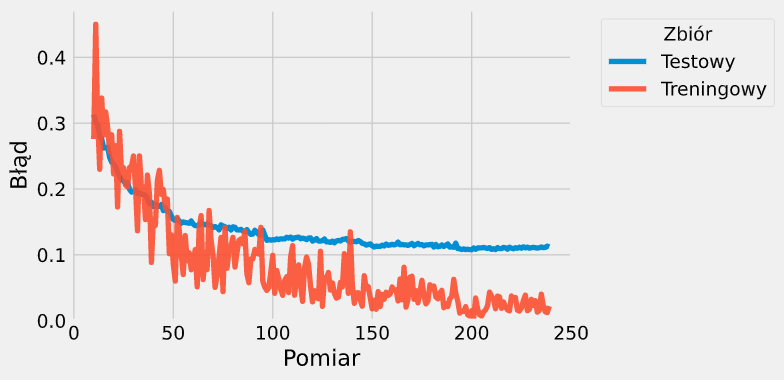
\includegraphics[width=\textwidth]{hidden_err_512.png}
	\label{fig:res15}
\end{figure}
\begin{figure}[H]
	\centering
	\caption{Zachowanie funkcji błędu dla 2048 neuronów}
	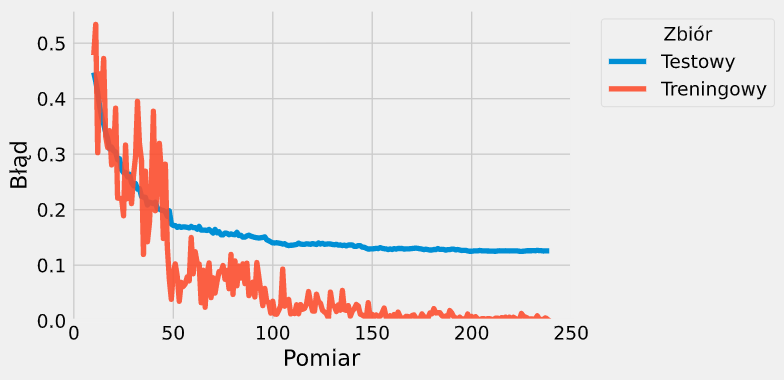
\includegraphics[width=\textwidth]{hidden_err_2048.png}
	\label{fig:res16}
\end{figure}

\begin{table}[H]
	\caption{Średnia maksymalna dokładność w zależności od wielkości warstwy ukrytej}
	\label{tabela-res-11}
	\centering
	\begin{tabular}{rrr}
		\toprule
		Neurony & Dokładność [\%] \\
		\midrule
		16      & 94.48              \\
		128     & 96.99              \\
		512     & 97.24              \\
		2048    & \textbf{97.54}     \\
		\bottomrule
	\end{tabular}
\end{table}

\subsubsection*{Wnioski}

Z otrzymanych wyników, widocznych na wykresach~\ref{fig:res11},~\ref{fig:res12} oraz tabeli~\ref{tabela-res-11}, wynika że większa ilość neuronów w warstwie ukrytej poprawia dokładność modelu, większa ilość parametrów pozwala na lepsze dopasowanie do danych. Uzyskane wyniki dla wielkości 128, 512 i 2048 są do siebie zbliżone, widać jednak spadek dla mniejszej warstwy (16 neuronów). Najlepszą dokładność uzyskał model z warstwą wielkości 2048, jednak na wykresach~\ref{fig:res16} i~\ref{fig:res15} można zauważyć, że błąd treningowy dla dla tych wielkości spada prawie do 0 co może świadczyć o zbytnim dopasowaniu do danych treningowych i predyspozycji do przeuczenia. W przeprowadzonych eksperymentach błąd testowy nie wzrastał w końcowych etapach uczenia, co wyklucza przeuczenie przy założonej ilości epok. Na wykresie~\ref{fig:res13} można natomiast zauważyć, że błędy treningowy i testowy dla małej warstwy ukrytej są na bardzo podobnym poziomie, w przeciwieństwie do pozostałych wielkości, gdzie błąd treningowy jest trochę niższy od testowego. Dodatkową obserwacją jest krótszy czas obliczeń przy uczeniu mniejszych modeli, spowodowany mniejszą ilością parametrów do zaktualizowania oraz przemnożenia podczas ewaluacji.

\newpage
\subsection{Wpływ wielkości paczki na przebieg procesu uczenia}
\subsubsection*{Założenia}
\begin{table}[H]
	\caption{Stałe dla eksperymentu 2}
	\label{tabela-const-2}
	\centering
	\begin{tabular}{lr}
		\toprule
		Parametr                   & Wartość         \\
		\midrule
		Wielkość warstwy ukrytej & 128               \\
		Zakres wag                 & \($-0.5 -- 0.5$\) \\
		Współczynnik uczenia     & 0.01              \\
		Funkcja aktywacji          & ReLU              \\
		\bottomrule
	\end{tabular}
\end{table}

Zmienną w tym eksperymencie była wielkość paczki. Ilość przykładów przyjmowała wartości ze zbioru \(\{$1, 8, 32, 128, 1024$\}\)
\subsubsection*{Przebieg}

Podczas eksperymentu model został zainicjalizowany 10 razy dla każdej z badanych wartości oraz wyuczony, uzyskane wyniki zostały zapisane w postaci pliku .plk do dalszej analizy.

\subsubsection*{Wyniki}
\begin{figure}[H]
	\centering
	\caption{Dokładność modelu w zależności od wielkości paczki}
	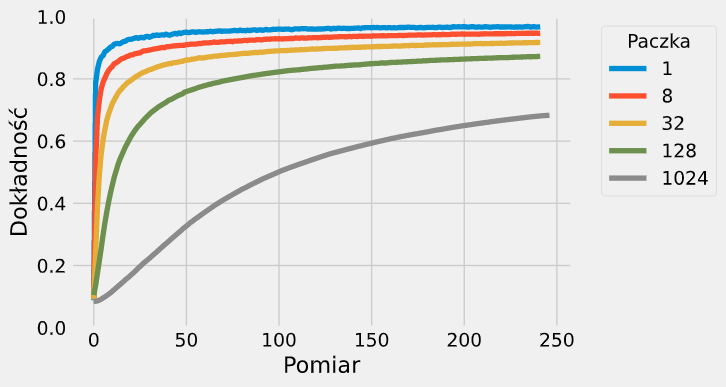
\includegraphics[width=\textwidth]{batch_acc.png}
	\label{fig:res21}
\end{figure}
\begin{figure}[H]
	\centering
	\caption{Dokładność modelu w końcowym etapie uczenia w zależności od wielkości paczki}
	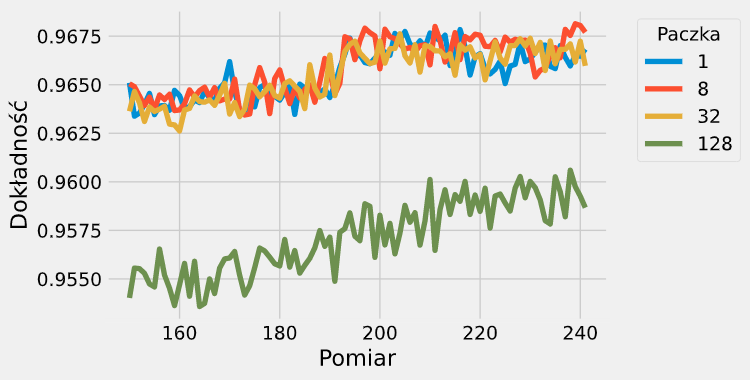
\includegraphics[width=\textwidth]{batch_acc_zoom.png}
	\label{fig:res22}
\end{figure}
\begin{figure}[H]
	\centering
	\caption{Zachowanie funkcji błędu dla paczki wielkości 1}
	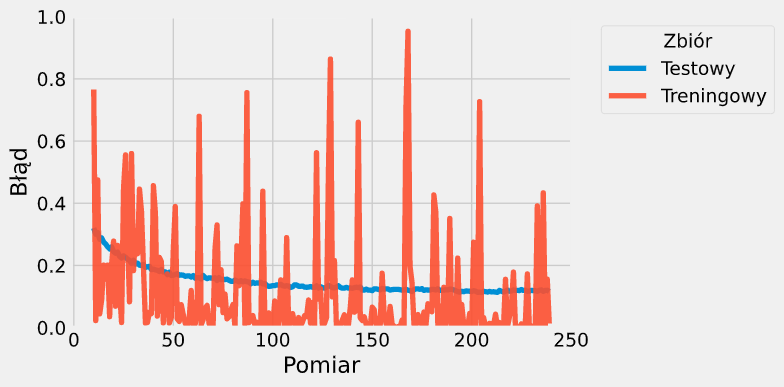
\includegraphics[width=\textwidth]{batch_err_1.png}
	\label{fig:res23}
\end{figure}
\begin{figure}[H]
	\centering
	\caption{Zachowanie funkcji błędu dla paczki wielkości 8}
	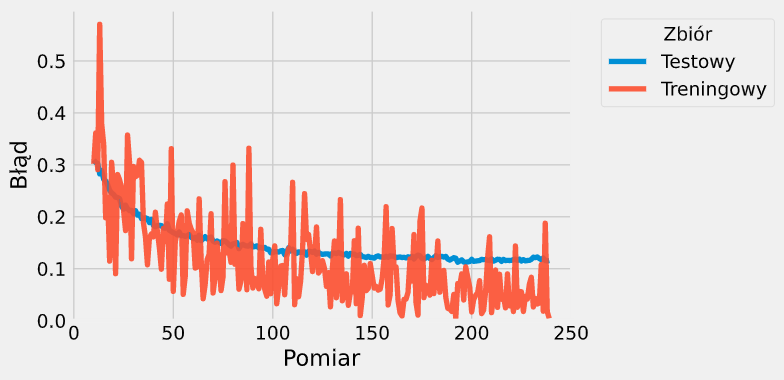
\includegraphics[width=\textwidth]{batch_err_8.png}
	\label{fig:res24}
\end{figure}
\begin{figure}[H]
	\centering
	\caption{Zachowanie funkcji błędu dla paczki wielkości 32}
	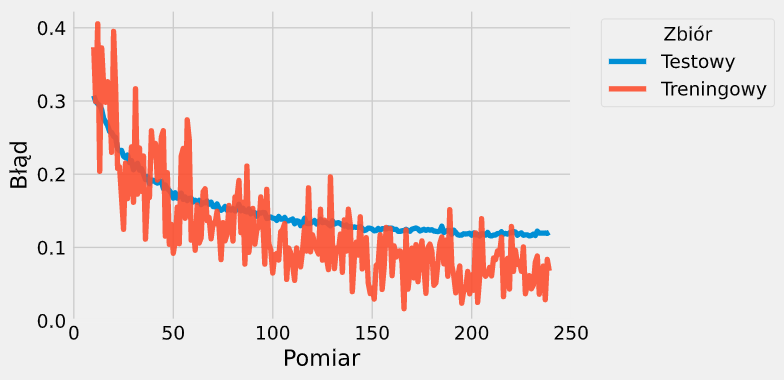
\includegraphics[width=\textwidth]{batch_err_32.png}
	\label{fig:res25}
\end{figure}
\begin{figure}[H]
	\centering
	\caption{Zachowanie funkcji błędu dla paczki wielkości 128}
	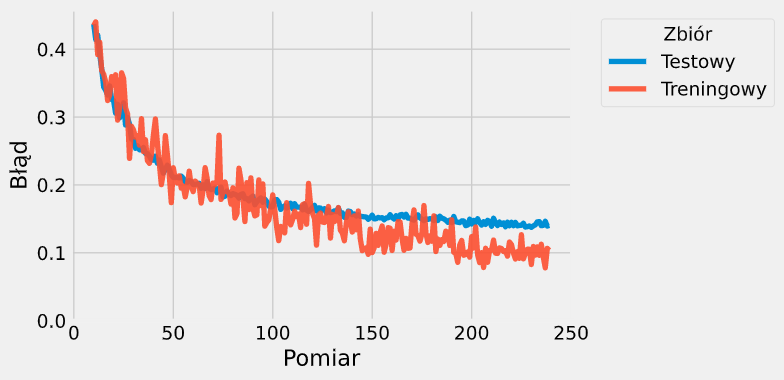
\includegraphics[width=\textwidth]{batch_err_128.png}
	\label{fig:res26}
\end{figure}
\begin{figure}[H]
	\centering
	\caption{Zachowanie funkcji błędu dla paczki wielkości 1024}
	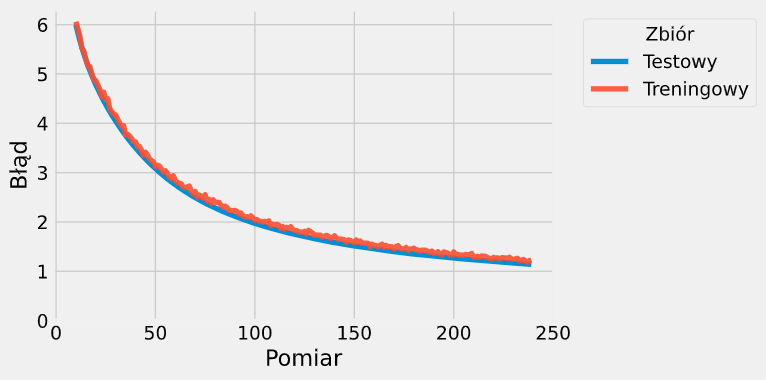
\includegraphics[width=\textwidth]{batch_err_1024.png}
	\label{fig:res27}
\end{figure}

\begin{table}[H]
	\caption{Średnia maksymalna dokładność w zależności od wielkości paczki}
	\label{tabela-res-21}
	\centering
	\begin{tabular}{rrr}
		\toprule
		Przykłady & Dokładność [\%] \\
		\midrule
		1          & 97.00              \\
		8          & \textbf{97.04}     \\
		32         & 96.99              \\
		128        & 96.32              \\
		1024       & 25.98              \\
		\bottomrule
	\end{tabular}
\end{table}

\subsubsection*{Wnioski}

Z otrzymanych wyników, widocznych na wykresach~\ref{fig:res21},~\ref{fig:res22} oraz tabeli~\ref{tabela-res-21}, wynika że małe wielkości paczki skutkują lepszą dokładnością modelu. Używanie za dużej paczki, jak widać w przypadku wielkości 1024, uniemożliwia wyuczenie. Po przeprowadzeniu dodatkowych badań okazało się jednak, że te wyniki są spowodowane przyjętym współczynnikiem uczenia, dla odpowiednio dobranych wartości alpha, mniejszych dla większych wielkości paczki, wyniki dla odpowiednio dobranych współczynników uczenia były zbliżone dla wszystkich rozmiarów. Zaletą mniejszych paczek, widoczną na wykresach~\ref{fig:res23},~\ref{fig:res24},~\ref{fig:res25},~\ref{fig:res26} i~\ref{fig:res27} jest wprowadzanie szumów do błędu treningowego, co przeciwdziała dążeniu do minimów lokalnych.
Dodatkową obserwacją jest krótszy czas obliczeń dla większych paczek spowodowany mniejszą ilością przeprowadzonych propagacji dla takiego samego zbioru uczącego.

\newpage
\subsection{Wpływ zakresu inicjalizacji wag na przebieg procesu uczenia}
\subsubsection*{Założenia}
\begin{table}[H]
	\caption{Stałe dla eksperymentu 3}
	\label{tabela-const-3}
	\centering
	\begin{tabular}{lr}
		\toprule
		Parametr                   & Wartość \\
		\midrule
		Wielkość warstwy ukrytej & 128       \\
		Wielkość paczki          & 32        \\
		Współczynnik uczenia     & 0.01      \\
		Funkcja aktywacji          & ReLU      \\
		\bottomrule
	\end{tabular}
\end{table}

Zmienną w tym eksperymencie był zakres inicjalizacji wag. Przedział inicjalizacji przyjmował wartości ze zbioru \(\{$0.0, -0.1 -- 0.1, -0.5 -- 0.5, -2.0 -- 2.0$\}\)
\subsubsection*{Przebieg}

Podczas eksperymentu model został zainicjalizowany 10 razy dla każdej z badanych wartości oraz wyuczony, uzyskane wyniki zostały zapisane w postaci pliku .plk do dalszej analizy.

\subsubsection*{Wyniki}
\begin{figure}[H]
	\centering
	\caption{Dokładność modelu w zależności od zakresu inicjalizacji wag}
	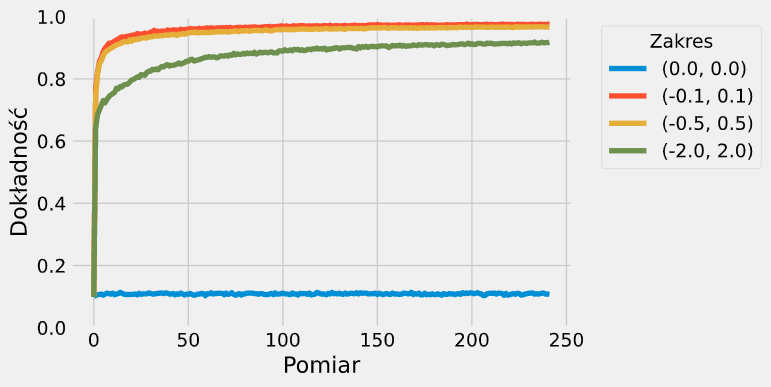
\includegraphics[width=\textwidth]{w_acc.png}
	\label{fig:res31}
\end{figure}
\begin{figure}[H]
	\centering
	\caption{Dokładność modelu w końcowym etapie uczenia w zależności od zakresu inicjalizacji wag}
	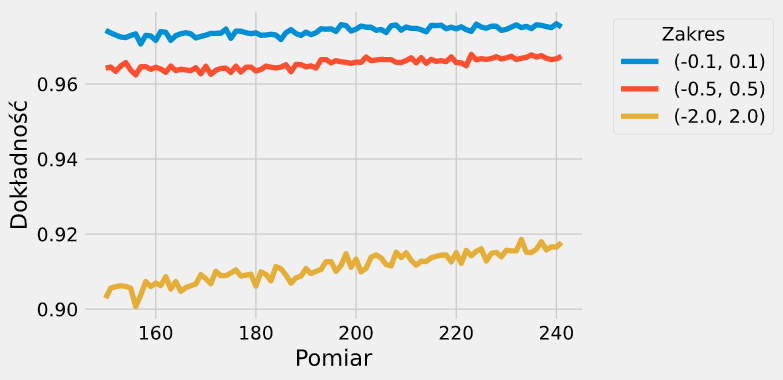
\includegraphics[width=\textwidth]{w_acc_zoom.png}
	\label{fig:res32}
\end{figure}
\begin{figure}[H]
	\centering
	\caption{Zachowanie funkcji błędu dla wag inicjalizowanych z zakresu \($0.0 -- 0.0$\)}
	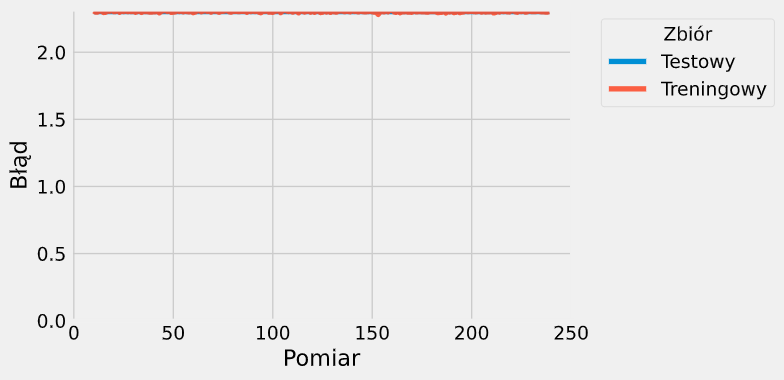
\includegraphics[width=\textwidth]{w_err_0.png}
	\label{fig:res33}
\end{figure}
\begin{figure}[H]
	\centering
	\caption{Zachowanie funkcji błędu dla wag inicjalizowanych z zakresu \($-0.1 -- 0.1$\)}
	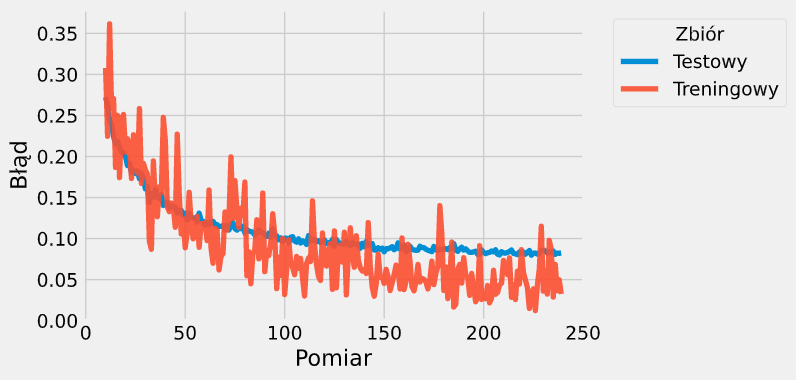
\includegraphics[width=\textwidth]{w_err_1.png}
	\label{fig:res34}
\end{figure}
\begin{figure}[H]
	\centering
	\caption{Zachowanie funkcji błędu dla wag inicjalizowanych z zakresu \($-0.5 -- 0.5$\)}
	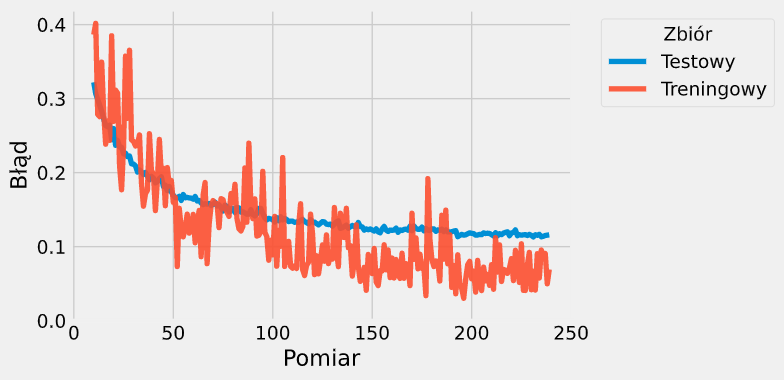
\includegraphics[width=\textwidth]{w_err_5.png}
	\label{fig:res35}
\end{figure}
\begin{figure}[H]
	\centering
	\caption{Zachowanie funkcji błędu dla wag inicjalizowanych z zakresu \($-2.0 -- 2.0$\)}
	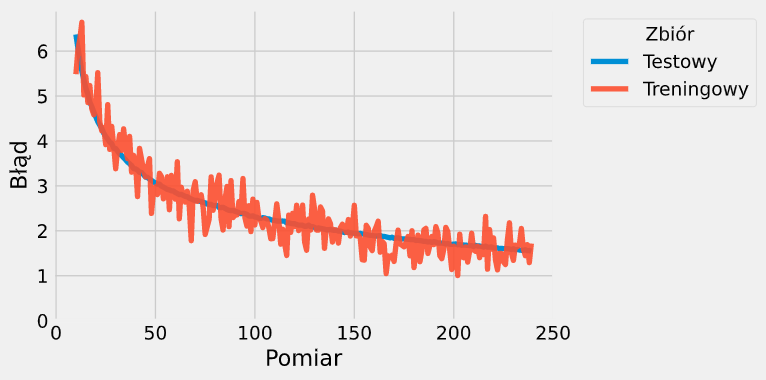
\includegraphics[width=\textwidth]{w_err_2.png}
	\label{fig:res36}
\end{figure}

\begin{table}[H]
	\caption{Średnia maksymalna dokładność w zależności od zakresu inicjalizacji wag}
	\label{tabela-res-31}
	\centering
	\begin{tabular}{rrr}
		\toprule
		Zakres            & Dokładność [\%] \\
		\midrule
		0.0               & 11.35              \\
		\($-0.1 -- 0.1$\) & \textbf{97.84}     \\
		\($-0.5 -- 0.5$\) & 96.99              \\
		\($-2.0 -- 2.0$\) & 92.14              \\
		\bottomrule
	\end{tabular}
\end{table}

\subsubsection*{Wnioski}

Z otrzymanych wyników, widocznych na wykresach~\ref{fig:res31},~\ref{fig:res32} oraz tabeli~\ref{tabela-res-31}, wynika że mniejsze zakresy inicjalizacji wag dają lepsze wyniki. Wyjątkiem jest inicjalizacja na 0, która skutkuje jednakowymi wartościami parametrów oraz ich aktualizacji co przekłada się na brak możliwości dopasowania do danych. Duże wartości powodują wolniejsze zbieganie oraz niższa dokładność końcową.

\newpage
\subsection{Wpływ wartości współczynnika alpha na przebieg procesu uczenia}
\subsubsection*{Założenia}
\begin{table}[H]
	\caption{Stałe dla eksperymentu 4}
	\label{tabela-const-4}
	\centering
	\begin{tabular}{lr}
		\toprule
		Parametr                   & Wartość         \\
		\midrule
		Wielkość warstwy ukrytej & 128               \\
		Wielkość paczki          & 32                \\
		Zakres wag                 & \($-0.5 -- 0.5$\) \\
		Funkcja aktywacji          & ReLU              \\
		\bottomrule
	\end{tabular}
\end{table}

Zmienną w tym eksperymencie był współczynnik uczenia. Przyjmował wartości ze zbioru \(\{$0.0001, 0.001, 0.01, 0.1, 1.0,$\}\)
\subsubsection*{Przebieg}

Podczas eksperymentu model został zainicjalizowany 10 razy dla każdej z badanych wartości oraz wyuczony, uzyskane wyniki zostały zapisane w postaci pliku .plk do dalszej analizy.

\subsubsection*{Wyniki}
\begin{figure}[H]
	\centering
	\caption{Dokładność modelu w zależności od współczynnika uczenia}
	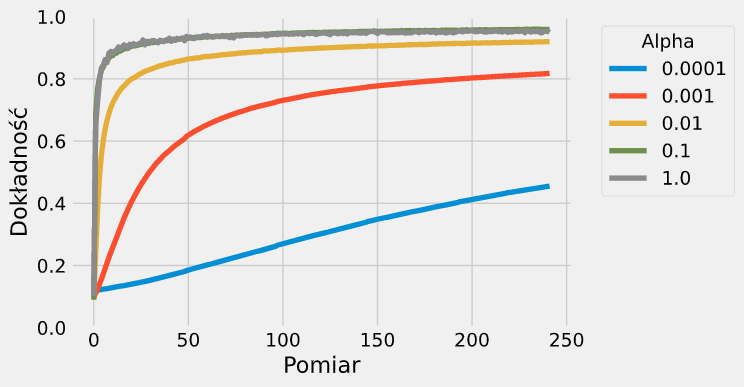
\includegraphics[width=\textwidth]{alpha_acc.png}
	\label{fig:res41}
\end{figure}
\begin{figure}[H]
	\centering
	\caption{Dokładność modelu w końcowym etapie uczenia w zależności od współczynnika uczenia}
	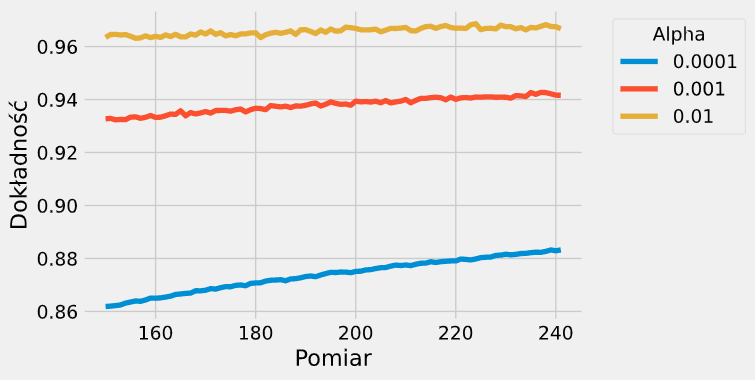
\includegraphics[width=\textwidth]{alpha_acc_zoom.png}
	\label{fig:res42}
\end{figure}
\begin{figure}[H]
	\centering
	\caption{Zachowanie funkcji błędu dla parametru alpha o wartości 0.0001}
	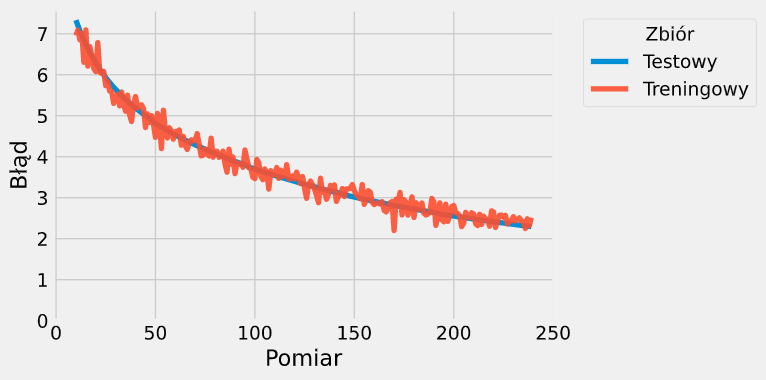
\includegraphics[width=\textwidth]{alpha_err_00001.png}
	\label{fig:res43}
\end{figure}
\begin{figure}[H]
	\centering
	\caption{Zachowanie funkcji błędu dla parametru alpha o wartości 0.001}
	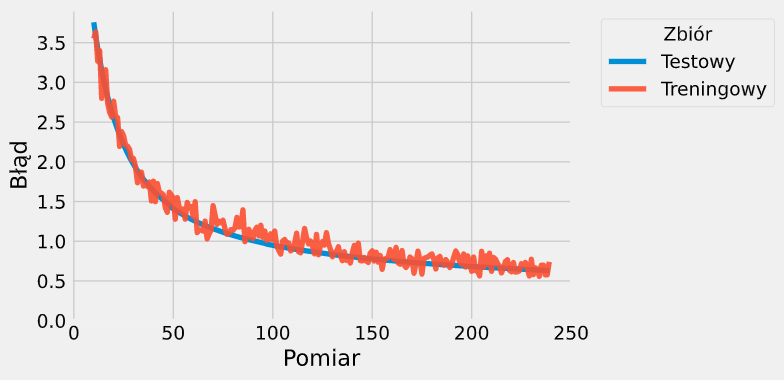
\includegraphics[width=\textwidth]{alpha_err_0001.png}
	\label{fig:res44}
\end{figure}
\begin{figure}[H]
	\centering
	\caption{Zachowanie funkcji błędu dla parametru alpha o wartości 0.01}
	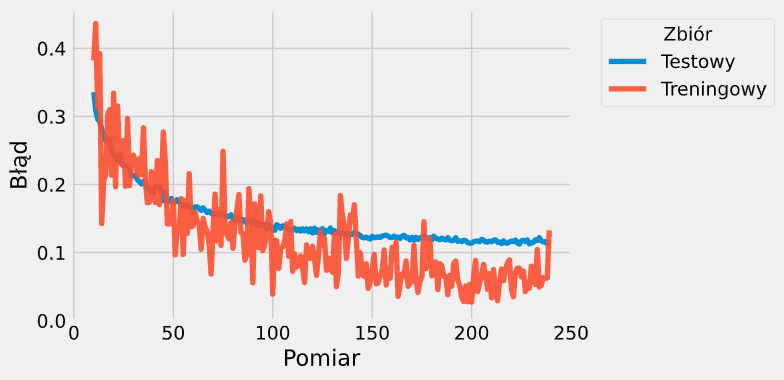
\includegraphics[width=\textwidth]{alpha_err_001.png}
	\label{fig:res45}
\end{figure}
\begin{figure}[H]
	\centering
	\caption{Zachowanie funkcji błędu dla parametru alpha o wartości 0.1}
	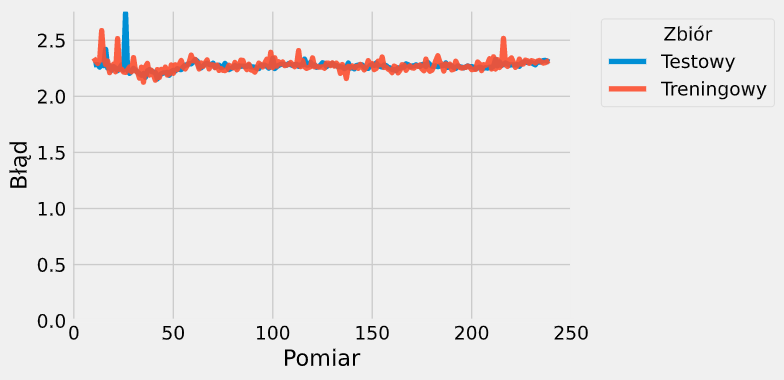
\includegraphics[width=\textwidth]{alpha_err_01.png}
	\label{fig:res46}
\end{figure}
\begin{figure}[H]
	\centering
	\caption{Zachowanie funkcji błędu dla parametru alpha o wartości 1.0}
	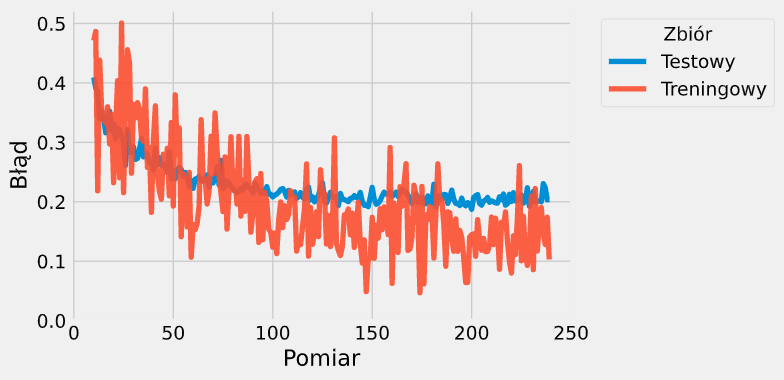
\includegraphics[width=\textwidth]{alpha_err_1.png}
	\label{fig:res47}
\end{figure}


\begin{table}[H]
	\caption{Średnia maksymalna dokładność w zależności od współczynnika uczenia}
	\label{tabela-res-41}
	\centering
	\begin{tabular}{rrr}
		\toprule
		Alpha  & Dokładność [\%] \\
		\midrule
		0.0001 & 88.37              \\
		0.0010 & 94.40              \\
		0.0100 & \textbf{97.06}     \\
		0.1000 & 23.84              \\
		1.0000 & 11.45              \\
		\bottomrule
	\end{tabular}
\end{table}

\subsubsection*{Wnioski}

Z otrzymanych wyników, widocznych na wykresach~\ref{fig:res41},~\ref{fig:res42} oraz tabeli~\ref{tabela-res-41}, wynika że duże wartości współczynnika alpha uniemożliwiają wyuczenie, jest to najprawdopodobniej spowodowane przeskakiwaniem wszelkich minimów przy tak dużych aktualizacjach parametrów. Bardzo małe wartości alpha nałożone od samego początku uczenia skutkują natomiast bardzo powolnymi poprawami wyników i prawdopodobnie utykaniem w minimach lokalnych co przekłada się na niższą końcową dokładność modelu. Na wykresach~\ref{fig:res43},~\ref{fig:res44} i~\ref{fig:res45} widać, że mniejsze wartości alpha wygładzają błąd treningowy.

\newpage
\subsection{Wpływ użytej funkcji aktywacyjnej na przebieg procesu uczenia}
\subsubsection*{Założenia}
\begin{table}[H]
	\caption{Stałe dla eksperymentu 5}
	\label{tabela-const-5}
	\centering
	\begin{tabular}{lr}
		\toprule
		Parametr                   & Wartość         \\
		\midrule
		Wielkość warstwy ukrytej & 128               \\
		Wielkość paczki          & 32                \\
		Zakres wag                 & \($-0.5 -- 0.5$\) \\
		Współczynnik uczenia     & 0.01              \\
		\bottomrule
	\end{tabular}
\end{table}

Zmienną w tym eksperymencie była funkcja aktywacji. Przetestowane zostały funkcje Sigmoidalna oraz ReLU.
\subsubsection*{Przebieg}

Podczas eksperymentu model został zainicjalizowany 10 razy dla każdej z badanych wartości oraz wyuczony, uzyskane wyniki zostały zapisane w postaci pliku .plk do dalszej analizy.

\subsubsection*{Wyniki}
\begin{figure}[H]
	\centering
	\caption{Dokładność modelu w zależności od funkcji aktywacji}
	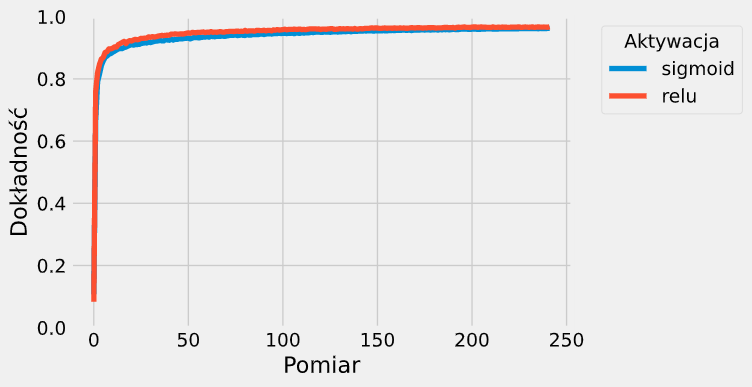
\includegraphics[width=\textwidth]{activation_acc.png}
	\label{fig:res51}
\end{figure}
\begin{figure}[H]
	\centering
	\caption{Dokładność modelu w końcowym etapie uczenia w zależności od funkcji aktywacji}
	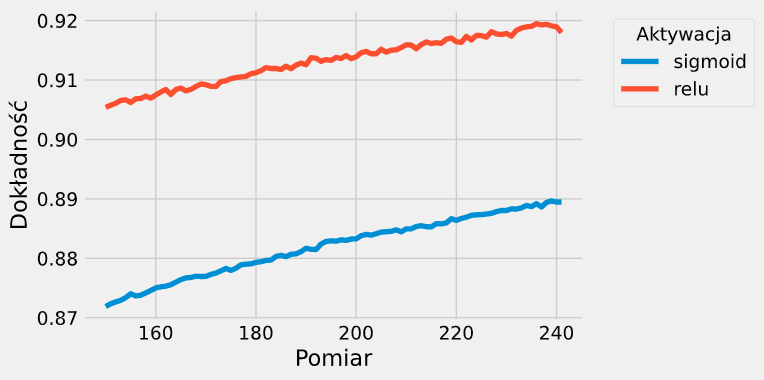
\includegraphics[width=\textwidth]{activation_acc_zoom.png}
	\label{fig:res52}
\end{figure}
\begin{figure}[H]
	\centering
	\caption{Zachowanie funkcji błędu dla funkcji aktywacji Sigmoidalnej}
	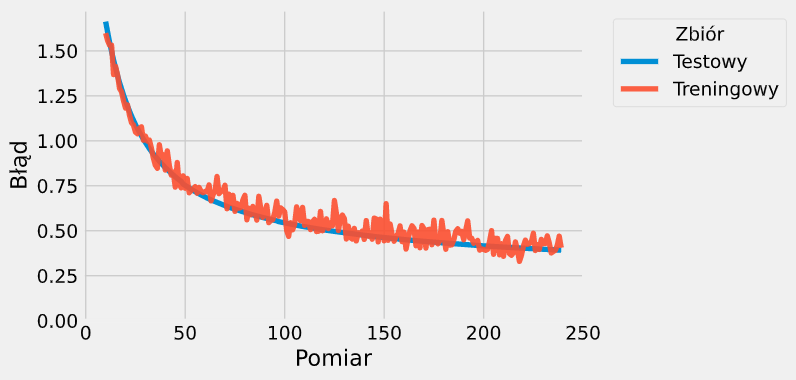
\includegraphics[width=\textwidth]{activation_err_sig.png}
	\label{fig:res53}
\end{figure}
\begin{figure}[H]
	\centering
	\caption{Zachowanie funkcji błędu dla funkcji aktywacji ReLU}
	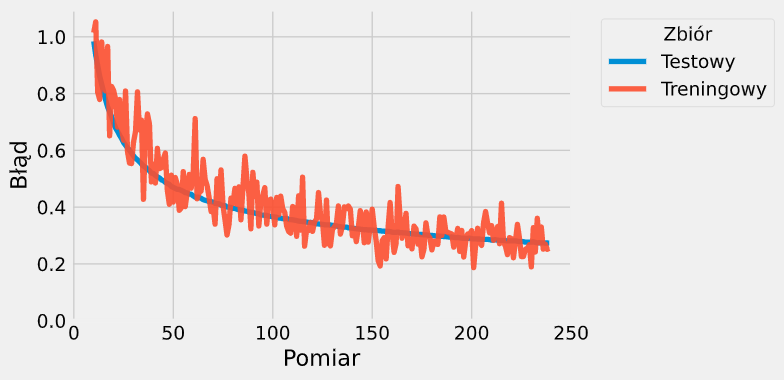
\includegraphics[width=\textwidth]{activation_err_relu.png}
	\label{fig:res54}
\end{figure}

\begin{table}[H]
	\caption{Średnia maksymalna dokładność w zależności od funkcji aktywacji}
	\label{tabela-res-51}
	\centering
	\begin{tabular}{rrr}
		\toprule
		Funkcja & Dokładność [\%] \\
		\midrule
		Sigmoid & 96.39              \\
		ReLU    & \textbf{96.94}     \\
		\bottomrule
	\end{tabular}
\end{table}

\subsubsection*{Wnioski}

Z otrzymanych wyników, widocznych na wykresach~\ref{fig:res51},~\ref{fig:res52} oraz tabeli~\ref{tabela-res-51}, wynika że funkcja ReLU daje lepsze wyniki. Używanie funkcji ReLU jest mniej kosztowne obliczeniowo, co dodatkowo przyspiesza trening.


\newpage
\section{Wnioski}

\begin{itemize}
	\item Wielowarstwowe sieci neuronowe pozwalają na modelowanie nieliniowych funkcji.
	\item Powtarzającym się motywem była korelacja niższego błędu treningowego niż testowy dla lepszych konfiguracji hiperparametrów. Może to oznaczać po prostu lepsze dopasowanie do danych oraz to, że MNIST jest na tyle prostym zbiorem danych, że prawie zerowy błąd na zborze uczącym nie implikuje przeuczenia, lecz dobra generalizację.
	\item Przy połączeniu wszystkich najlepszych hiperparametrów otrzymanych z eksperymentów, model uzyskuje dokładność \($>98\%$\).
	\item Hiperparametry wpływają na siebie nawzajem, podczas badań najbardziej wyraźny był wpływ współczynnika uczenia na możliwość używania większych wielkości paczki.
	\item Odpowiednie ustawienie hiperparametrów może znacząco przyspieszyć proces uczenia.
	\item Architektura sieci ma duży wpływ na jej możliwości i wydajność.
\end{itemize}

\end{document}